\section*{Introduction}
Dans ce chapitre, nous expliquerons en détail les méthodes que nous avons
employées pour l’ADT.\\
Pour commencer, nous exposerons une description de la notation de la batterie
ainsi qu’une modélisation de celle-ci pour la représentation des données
rythmiques en arbres syntaxiques. Nous poursuivrons avec une présentation de
qparse\footnote{https://qparse.gitlabpages.inria.fr/}, un outil de
transcription qui est développé à l'Inria, l'Université de Nagoya et plusieurs
développeurs au sein du laboratoire Cedric au CNAM.

Enfin, nous présenterons les \textbf{formes rythmiques}, <flo>une
représentation
théorique qui permet…</flo> 

\section{La notation de la batterie}
\label{notation_batterie}
Pour la transcription, j’ai choisi d’utiliser une notation inspirée du recueil
de pièces pour batterie de J.-F. Juskowiak \cite{jusko} et des méthodes de
batterie Agostini \cite{ago_meth_3}, car je trouve la position des éléments
cohérente et intuitive (voir section \ref{hauteurs}).\newpage

%\subsection*{Les hauteurs et les têtes de notes}
%\label{hauteurs}
\begin{figure}[h]
\centering
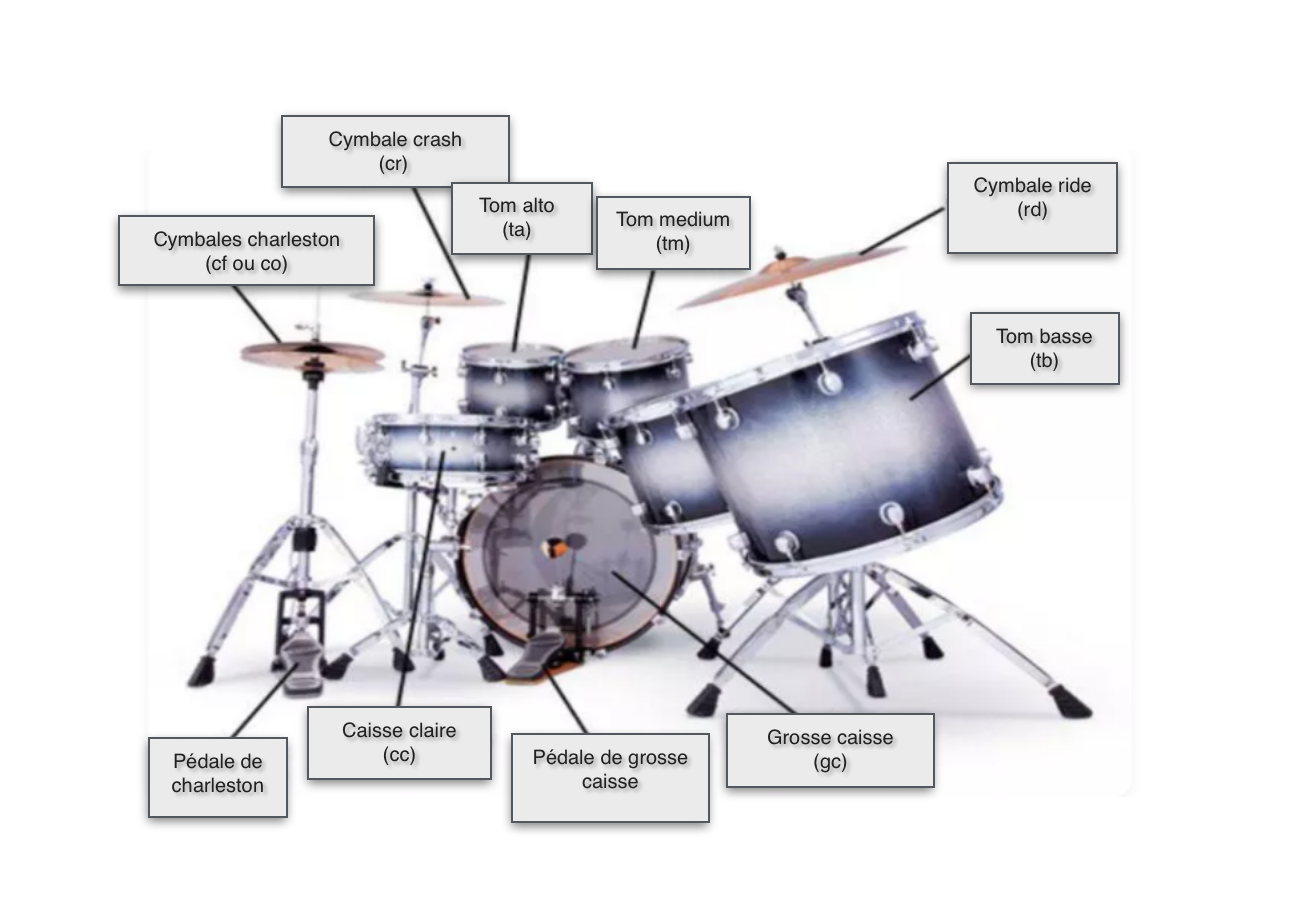
\includegraphics[height=69mm, width=115mm]{
z_images/3_methodes/0_notation_de_la_batterie/batterie.png}
\caption{Les instruments de la batterie}
\label{instru_batt}
\end{figure}

\begin{figure}[!h]
\centering
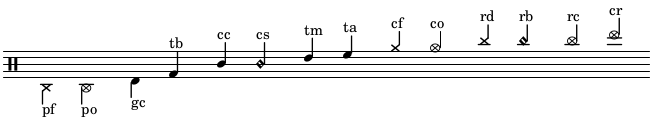
\includegraphics[height=25mm, width=130mm]{
z_images/3_methodes/0_notation_de_la_batterie/2_hauteurs_et_tete_de_notes.png}
\caption{Hauteur et têtes de notes}
\label{haut}
\end{figure}

\begin{table}[h]
\centering
\begin{tabular}{|c|c|c|} \hline
Noms figure \ref{instru_batt} & codes figure \ref{haut}  & référence \\ \hline
Pédale de charleston & pf ou po & charley fermé ou ouvert au pied \\
Grosse caisse & gc & grosse caisse \\
Tom basse & tb & tom basse \\
Caisse claire & cc & caisse claire \\
Tom médium & tm & tom médium \\
Tom alto & ta & tom alto \\
Cymbales charleston & cf ou co & charley fermé ou ouvert à la main \\
Cymbales ride & rd & ride \\
Cymbales crash & cr & crash \\ \hline
	\end{tabular}
	\caption{Noms des instruments de la batterie}
	\label{nom_instru_batt}
\end{table}\newpage
La figure \ref{instru_batt}\footnote{Source : \url{
https://www.superprof.fr/blog/composition-instrument-percussion/}} montre une
batterie standard avec tous les instruments habituellement présent sur une
batterie et la figure \ref{haut} donne leur représentation sur une partition.

Le tableau \ref{nom_instru_batt} donne dans l’ordre :
\begin{enumerate}
    \item les noms des instruments sur la figure \ref{instru_batt} ;
    \item leurs codes respectifs dans la figure \ref{haut} ;
    \item les noms que j’utiliserai dans le présent document pour y référer.
\end{enumerate}
Les figures \ref{instru_batt}, \ref{haut} et le tableau \ref{nom_instru_batt}
peuvent aider à comprendre pourquoi je trouve la notation agostinienne
cohérente et intuitive.

En effet, les hauteurs sur la portée représentent :
\begin{enumerate}
	\item La hauteur physique des instruments :\\
	La caisse claire est centrale sur la portée et sur la batterie (au niveau
    de la ceinture, elle conditionne l’écart entre les pédales et aussi la
    position de tous les instruments basiques d’une batterie).\\
	Tout ce qui en-dessous de la caisse claire sur la portée est en dessous de
    la caisse claire sur la batterie (pédales, tom basse) ;\\
	Tout ce qui est au-dessus de la caisse claire sur la portée, l’est aussi
    sur la batterie.\\
	\item La hauteur des instruments en terme de fréquences :\\
	Sauf pour le charley au pied et si l’on sépare en trois groupes
    (grosse caisse, toms et cymbales), de bas en haut, les instruments vont du
    plus grave au plus aigu.
\end{enumerate}

\subsection*{Les durées}
\label{hho}
Comme nous venons de la voir, la majorité des instruments de la batterie sont
représentés par les têtes des notes. De plus, le seul instrument dont le son
peut être arrêté de manière quantifiée et dont la durée sonore nous intéresse
est le charley\footnote{Je ne prendrais pas en compte l’arrêt des cymbales à la
main car ce phénomène n’existe pas dans les fichiers MIDI.}.
\florent{certaines têtes de notes vides alors que leur durée n'est pas celle
des blanches? expliquer les différences avec la notation conventionnelle cf
1.4}

Par conséquent :
\begin{enumerate}
    \item les durées — sauf pour le charley — représenterons un écart temporel
        entre les notes et non une durée sonore et elles pourront donc être
        rallongée à l’aide de silences ;
    \item les symboles rythmiques concernant les têtes de note ne pourront pas
        être utilisés pour exprimer les durées. Cela est valable aussi pour la
        présence ou non de la hampe puisque ce phénomène n’existe qu’avec les
        têtes de notes de type cercle-vide (opposition blanche-ronde). L’usage
        des blanches existe dans certaines partitions de batterie
        \cite{system_drums} mais cela reste dans des cas très rares. Certains
        logiciels permettent de faire des blanches avec des symboles
        spécifiques à la batterie ou aux percussions mais leur lecture reste
        peu aisée et leur utilisation pour la batterie est rarissime.\\
\end{enumerate}

En résumé :
\begin{itemize}
    \item toutes les notes ont une hampe ;
    \item une notes dont la hampe n’a pas de crochet est toujours une noire ;
    \item à part pour le charley ouvert, les durées n’expriment pas la durée
        d’un son mais une distance temporelle entre deux notes.
    \item à part pour le charley ouvert, la durée d’une note peut être
        prolongée par un silence (exemple : une noire + un soupir pour exprimer
        une blanche)\\
\end{itemize}
La durée d’une note peut être prolongée par divers symboles :
\begin{itemize}
	\item Le point : il rallonge la durée d’une note de la moitié de sa valeur.
        Dans la deuxième note de l’exemple 3 de la figure \ref{point_liaison}
        est une noire pointée, elle vaut donc la durée d’une noire + une croche
        (ou de trois croche) ;
	\item La liaison : elle rallonge la durée de la première note de la durée
        de la deuxième. La deuxième note de l’exemple 4 de la figure
        \ref{point_liaison} est une croche qui est liée à une noire, sa durée
        est donc équivalente à celle d’une croche + une noire (ou de trois
        croches) ;
    \item les silences (pas pour les ouvertures de charley).
\end{itemize}

\begin{figure}[h]
	\centering
	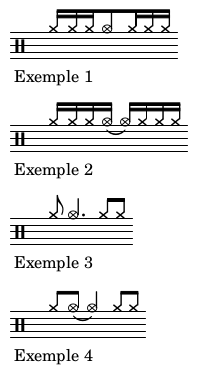
\includegraphics[height=80mm, width=40mm]{
    z_images/3_methodes/0_notation_de_la_batterie/3_point_et_liaison.png}
	\caption{Point et liaison}
	\label{point_liaison}
\end{figure}

Un autre élément concernant la notation des durées en batterie est la nécessité
de faire ressortir la pulsation\footnote{La position des temps} de la rendre
visuelle. La première chose à prendre en compte pour analyser la figure
\ref{point_liaison} est donc la nécessité de regrouper les notes par temps à
l’aide des ligatures. Le deuxième point est de s’arranger pour qu’il y ait une
indication visuelle au début de chaque temps.

\begin{itemize}
    \item Exemple 1 : l’ouverture de charley est quantifiée mais les notes ne
        sont pas regroupées par temps.
    \item Exemple 2 : Ici, la liaison permet de regrouper les notes par temps
        en obtenant le même rythme que dans l’exemple 1.
    \item Exemple 3 et exemple 4 : les deux exemples sont valables mais le
        deuxième est le plus souvent utilisé car la liaison donne un repair
        visuel sur le temps.\\
\end{itemize}

En cas de nécessité de prolonger la durée d’une note au-delà 
de son temps de départ (syncope) et si cette note ne correspond pas à une
ouverture de charley, elle sera prolongerée sur le temps suivant à l’aide de
silences dont le premier sera positionné sur le temps. Si la note syncopée est
une ouverture de charley, on privilégiera la liaison pour sa prolongation.

\subsection*{Les silences}
Les silences sont parfois utilisés pour noter les fermetures de charley (après
une ouverture). Les fermetures du charley sont notées soit par un silence
(correspondant à une fermeture de la pédale), soit par un écrasement de
l’ouverture par un autre coup de charley fermé, au pied ou à la main.

\begin{figure}[h]
	\centering
	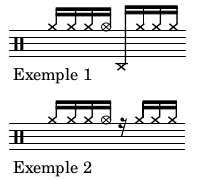
\includegraphics[height=40mm, width=40mm]{
    z_images/3_methodes/0_notation_de_la_batterie/5_silence_joue.png}
	\caption{Silence joué}
	\label{silence joue}
\end{figure}

L’écriture littérale de contenu MIDI peut ressembler à l’exemple 1 de la figure
\ref{silence joue}. Sur cet exemple, le son de l’ouverture de charley est
arrêté par une pression du pied sur la pédale et c’est ce que le batteur joue
dans les faits. Mais il apparaît intuitivement que le but de la première note
du deuxième temps n’est pas de générer un son de charley au pied mais
uniquement de stopper l’ouverture. La notation de l’exemple 2 de la figure
\ref{silence joue} serait donc préférable car elle représente mieux l’intention
de ce rythme et elle n’empiète pas sur une potentielle voix basse qui pourrait
le compléter (on évite une écriture surchargée).

Lorsqu’une note est un charley ouvert, il faudra donc prendre en compte la note
suivante pour l’écriture :
\begin{enumerate}
    \item si c’est un charley fermé joué à la main $\Rightarrow$ la note sera
        un charley fermé joué à la main (cf) ;
    \item si c’est un charley fermé joué au pied $\Rightarrow$ la note sera un
        silence.
\end{enumerate}
La deuxième règle sera soumise au cadre imposé par certaines
\textbf{formes rythmiques} pour lesquelles le charley joué au pied devra rester
tel quel. 

\subsection*{Les équivalences rythmiques}
Pour les instruments mélodiques, dans le cas de notes dont la durée de l’une à
l’autre est ininterrompue et si leur durée initiale est prolongée, seuls la
liaison et le point permettent des notations équivalente. Mais pour la
batterie et à part dans le cas des ouvertures de charley (voir section
\ref{hho}), seules comptent des dates de début (onsets) : la durée du son n’a
pas d’importance. L’usage des silences pour combler la distance rythmique entre
deux notes devient donc possible.

Cela pris en compte, et étant donné que les indications de durée dans les têtes
de notes sont peu recommandées (voir section \ref{hho}), l’écriture à l’aide de
silences sera privilégiée comme indication de durée sauf dans les cas où cela
reste impossible. Ce choix à pour but de n’avoir qu’une manière d’écrire toutes
les notes, quelles que soient leur tête de note (sauf pour le charley).

\begin{figure}[h]
	\centering
	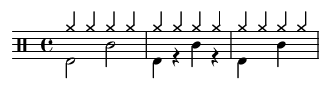
\includegraphics[height=20mm, width=75mm]{
    z_images/3_methodes/0_notation_de_la_batterie/6_equivalence.png}
	\caption{Équivalence}
	\label{equivalence}
\end{figure}

Sur la figure \ref{equivalence}, théoriquement, il faudra choisir la notation
de la deuxième mesure mais dans certains contextes, pour des raisons de
lisibilité ou de surcharge, la version sans les silences de la troisième mesure
pourra être choisie.

\subsection*{Les voix}
Pour les instruments mélodiques, un groupe de notes peut être organisé en
\emph{voix}, représentant des flots mélodiques joués en parallèle, avec une
synchronisation plus ou moins stricte \cite{SHIBATA2021262}
\cite{Guiomard-Kagan}.
% voir ref [15] ou [16] de SHIBATA….

En batterie, une voix est théoriquement l’ensemble des instruments qui, à eux
seuls, constituent une phrase rythmique. Mais en pratique, les instruments
peuvent aussi être divisés par voix dans le but de ne pas surcharger la
notation ou pour que leur disposition soit représentée sur la
partition (voir section \ref{notation_batterie}).
Les voix sont charactérisées par l’orientation des hampes et plus présicément
par les ligatures si les hampes sont dans la même direction (voir figure
\ref{afro_latin}).

\begin{figure}[h]
	\centering
	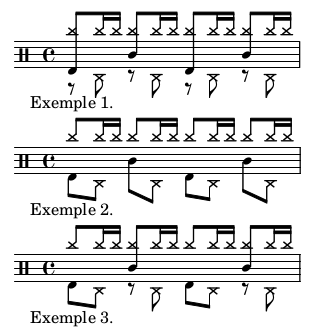
\includegraphics[height=65mm, width=60mm]{
    z_images/3_methodes/0_notation_de_la_batterie/7_voix.png}
	\caption{Séparation des voix}
	\label{sep_voix}
\end{figure}
Sur la figure \ref{sep_voix}, il faudra faire un choix entre les exemples 1, 2
et 3 qui sont trois façons équivalentes d’écrire le même rythme.
Ce choix se fera en fonction des instruments joués, de la nature plus ou moins
systèmatique de leurs phrasés, et des associations logiques entre les
instruments dans la distribution des rythmes sur la batterie (voir la section
\ref{sys_sep_voix}).

\subsection*{Les accentuations et les ghost-notes}
« Certaines notes dans une phrase musicale doivent, ainsi que les différentes
syllabes d’un mot, être accentuées avec plus ou moins de force, porter une
inflexion particulière. » \cite{danhauser}
\begin{figure}[h]
\centering
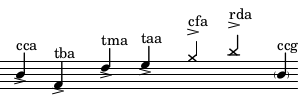
\includegraphics[height=25mm, width=75mm]{
z_images/3_methodes/0_notation_de_la_batterie/8_accents_et_ghost-notes_0.png}
\caption{Les accents et les ghost-notes}
\label{accents_et_gn}
\end{figure}

Théoriquement, tous les instruments peuvent être accentués (voir la section
\ref{velocite}), mais la figure \ref{accents_et_gn} représentent ceux dont les
accents ne demandent pas un grand niveau de maîtrise et sont presque toujours
bien articulés. En outre, les instruments qui ne sont pas représentés sur cette
figure ne sont presque jamais accentués dans les partitions et ne sont pas
présents de manière significative dans le GMD.

Les accents sont marqués par le symbole~«~>~». Ils sont positionnés au-dessus
des notes représentant des cymbales et en-dessous des notes représentant des
toms ou la caisse claire. Ce choix a été fait pour la partition de la figure
\ref{partition_ref} car elle est plus lisible ainsi, mais ces choix devront
être adaptés en fonction des différentes \textbf{formes rythmiques} reconnues
(voir la section \ref{systemes_methodes}). Par exemple, pour les
\textbf{formes rythmiques} jazz, les ligatures pour les toms et la caisse
claire seront dirigées vers le bas, il faudra donc mettre les symboles
d’accentuation correspondants au-dessus des têtes de notes.

La dernière note de la figure \ref{accents_et_gn} montre un exemple de notation
pour une ghost note jouée à la caisse claire. Une ghost note
\cite{lexique_drum} est une note de faible volume sonore mais jouée fermement.
Les ghost notes servent le plus souvent à donner le débit d’un rythme (ses
subdivisions) pour le rendre plus dansant (lui donner plus de « groove » ou de
« swing »). Le parenthésage a été choisi car il peut être utilisé sur n’importe
quelle note sans changer la tête de note.

Toutes les notes de la figure \ref{accents_et_gn} sont exposées en situation
réelle dans la figure \ref{exemple_acc_et_gn}. 
\begin{figure}[h]
\centering
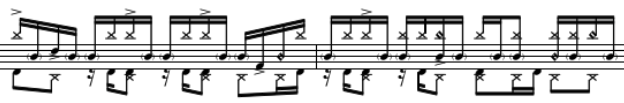
\includegraphics[height=20mm, width=110mm]{
z_images/3_methodes/0_notation_de_la_batterie/8_accents_et_ghost-notes_1.png}
\caption{Exemple pour les accentuations et les ghost-notes}
\label{exemple_acc_et_gn}
\end{figure}

\subsection*{Les flas}
Le fla est appogiature qui consiste à jouer deux coups presque simultanés dont
le premier est une ghost note et le deuxième une note normale ou accentuée.
\begin{figure}[h]
    \centering
    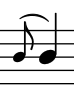
\includegraphics[height=10mm, width=8mm]{
    z_images/3_methodes/0_notation_de_la_batterie/fla_def.png}
    \caption{Définition du fla}
\end{figure}

\section{La transcription manuelle}
Mis à part les figures du chapitre 1 et certains exemples d’analyses de la
section \ref{analyses_et_TM}, toutes les partitions et figures de ce document
ont généré avec lilypond\footnote{\url{http://lilypond.org/index.fr.html}}.\\

\subsection*{Présentation de lilypond}
« LilyPond est un logiciel de gravure musicale, destiné à produire des
partitions de qualité optimale. Ce projet apporte à l’édition musicale
informatisée l’esthétique typographique de la gravure traditionnelle. LilyPond
est un logiciel libre rattaché au projet GNU. »\\

En raison de :
\begin{itemize}
    \item notation agostini
    \item grande liberté de choix
    \item …
\end{itemize}

Lilypond est actuellement le meilleur de logiciel de gravure musicale pour la
batterie.

\begin{figure}[h]
    \centering
    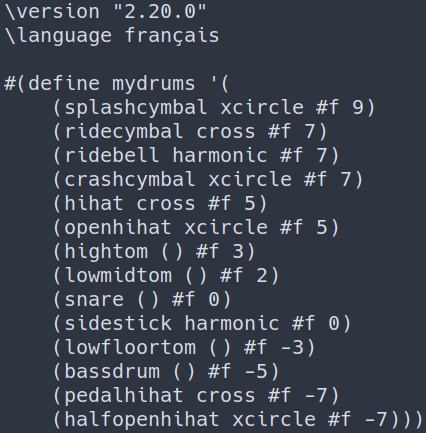
\includegraphics[height=40mm, width=30mm]{
    z_images/3_methodes/transcription_manuelle/drum_perso_1}
    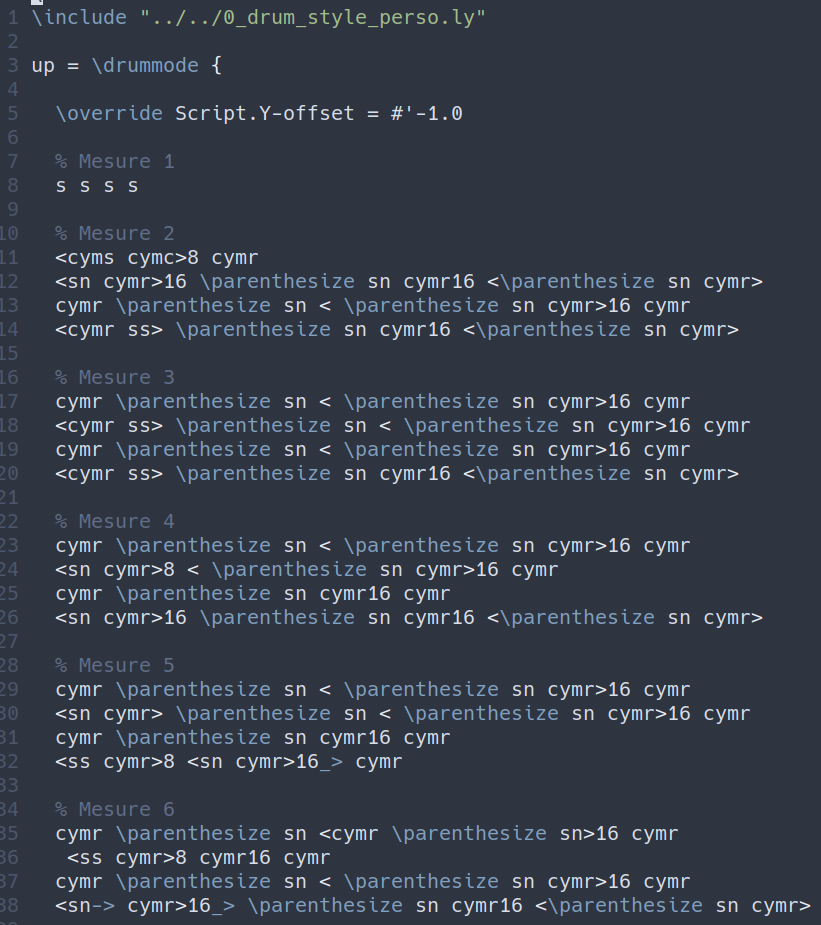
\includegraphics[height=70mm, width=50mm]{
    z_images/3_methodes/transcription_manuelle/extrait_code.png}
    \caption{lilypond — extraits de code}
    \label{extrait_code}
\end{figure}

Sur la figure \ref{extrait_code} :
\begin{itemize}
    \item à gauche : configuration aménagée pour la notation de type agostini.
    \item à droite : le début de code mesure par mesure pour la voix haute
        d’une partition (en haut du fichier, inclusion du fichier de config)
\end{itemize}

\begin{figure}[h]
    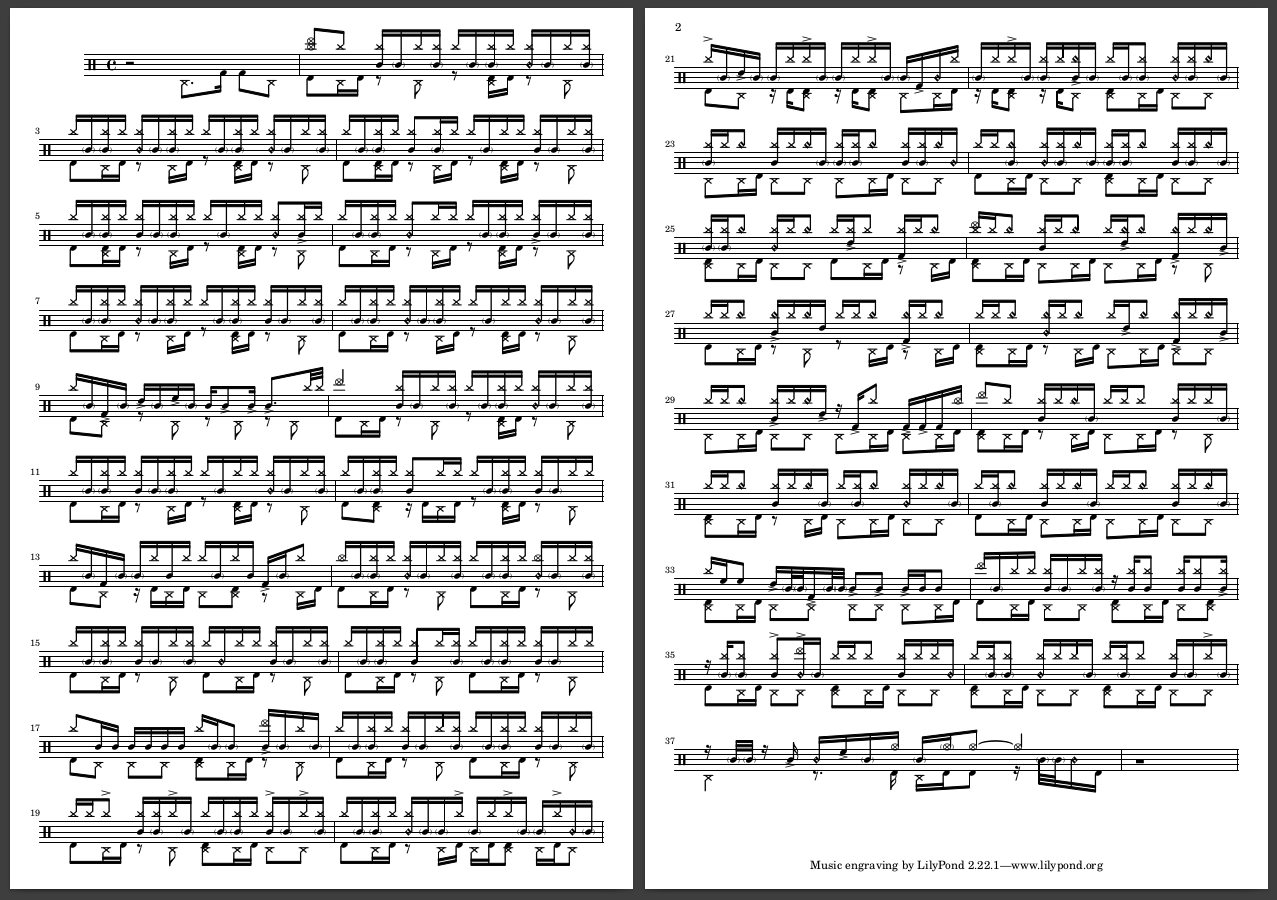
\includegraphics[height=120mm, width=160mm]{
    z_images/4_experimentations/1_analyses/3_partition.png}
    \caption{lilypond — transcription manuelle}
	\label{partition_ref}
\end{figure}

La partition de la figure \ref{partition_ref} est le résultat du code de la
figure \ref{extrait_code} (la totalité du code est mis en annexe et est
accessible sur le git). Cette partition a été totalement transcrite
manuellement avec lilypond par analyse des fichiers MIDI et audio
correspondants.

\begin{itemize}
    \item difficultés principales : trouver une application permettant de
        choisir librement la notation de la batterie. Lylipond le permet mais
        beaucoup de recherches ont été nécessaires pour comprendre l’ensemble
        des fonctionnalités permettant de faire fonctionner la notation
        « agostinienne » ainsi que les diverses subtilités de notations
        (accents, ghost-notes, flas, …).\\
        lylipond reste néanmoins un choix très agréable, une fois ces
        difficultés surmontées.
    \item Écrire la partition de la figure \ref{partition_ref} m’a pris
        beaucoup de temps car j’ai dû chercher comment écrire chaque nouvel
        évènement mais les autres transcriptions ont été beaucoup plus rapide
        et très aisées.
    \item Même si cela représente un investissement au départ, je recommande
        lylipond pour écrire la batterie et je pense que c’est meilleur outil
        pour cette tâche pour le moment. On peut configurer absolument tout.
    \item dans les autres logiciel d’édition de type musescore, la batterie
        est toujours confiné au système de notation américain.
    \item pour une comparaison entre système américain et système agostinien,
        voir section \ref{flas} est comparer les notations TM (agostinien) et
        TA (américain).
\end{itemize}


\section{Modélisation pour la transcription}
\label{modelisation_transcription}
\subsection*{Les pitchs}
\begin{table}[h]
	\centering
	\begin{tabular}{|c|c|c|} \hline
		Codes & Instruments & Pitchs \\ \hline
		cf & charley-main-fermé & 22, 42 \\
		co & charley-main-ouvert & 26 \\
		pf & charley-pied-fermé & 44 \\
		rd & ride & 51 \\
		rb & ride-cloche (bell) & 53 \\
		rc & ride-crash & 59 \\
		cr & crash & 55 \\
		cc & caisse claire & 38, 40 \\
		cs & cross-stick & 37 \\
		ta & tom-alto & 48, 50 \\
		tm & tom-medium & 45, 47 \\
		tb & tom-basse & 43, 58 \\
		gc & grosse caisse & 36 \\ \hline
	\end{tabular}
	\caption{Codes, identités et pitchs des instruments}
	\label{pitchs_instru}
\end{table}
Le tableau \ref{pitchs_instru} présente dans l’ordre, les codes des
instruments, leur identité (instrument ou parti d’un instrument — joué avec les
mains ou avec les pieds), le ou les pitchs qui lui sont associés.

Plusieurs pitchs peuvent parfois désigner le même instrument afin de pouvoir
supporter des kits de batterie plus larges (avec par exemple plusieurs toms
basses qui n’auraient pas tous exactement la même sonorité) ou simplement de
styles différents (pour chaque kits standard, ce sont les mêmes intruments mais
de styles différents)\footnote{Par exemple, les peaux des
toms jazz raisonnent alors que les toms rock sont mat.}.
J’ai regroupé les pitchs des différents types d’un même instrument dans une
seule ligne du tableau portant le nom du type de cet instrument. Ainsi,
plusieurs toms basses différents dans les données MIDI deviennent tous un tom
basse d’une batterie standard et la partition finale pourra être jouée sur
n’importe quel kit de batterie standard.

Malgré le large panel de pitchs disponibles, il semblerait qu’aucun pitch ne
désigne le charley ouvert joué au pied (« po » de la figure \ref{haut}).
Pourtant, dans la batterie moderne, plusieurs rythmes ne peuvent fournir le son
du charley ouvert qu’avec le pied car les mains jouent autre chose en même
temps. Cela doit en partie être dû à l’utilisation des boîtes à rythmes
en MAO qui ne nécessitent pas de faire des choix conditionnés par les
limitations humaines (2 pieds, 2 mains, et beaucoup plus d’instruments…)

\subsection*{La vélocité} \label{velocite}
La vélocité déterminera si les notes sont accentuées ou sont des ghost notes.
Pour les codes, je propose d’ajouter un suffix (« a » pour accent et «g» pour
ghost note) à la fin du code d’une note accentuée ou d’une ghost note.
Les choix pour déterminer si les notes sont accentuées ou sont des ghost notes
seront donnée dans la section \ref{partition_entiere}.

\subsection*{Les arbres de rythmes}
Les arbres de rythmes représentent un rythme dont les possibilités de notation
sur une partition sont théoriquement multiples. Les branchements sont des
divisions d’interval temporel, les feuilles sont des évènements musicaux
commençant au début de l’interval \cite{Laurson1996PatchWorkA}
\cite{Bresson_openmusicvisual} .\\
Voici une représentation qui fonctionne avec les 3 exemples de la figure
\ref{sep_voix} en arbre de rythmes avec les codes de chaque instrument :
\begin{figure}[h]
	\Tree[ [ [rd\\gc ][ [rd\\pf ][rd ]]]
	[ [rd\\cc ][ [rd\\pf ][rd ]]]
	[ [rd\\gc ][ [rd\\pf ][rd ]]]
	[ [rd\\cc ][ [rd\\pf ][rd ]]] ]
\end{figure}

Ci-dessous, le même arbre dont les codes des instruments sont remplacés par
leurs données MIDI respectives :
\begin{figure}[h]
	\Tree[ [ [51\\36 ][ [51\\44 ][51 ]]]
	[ [51\\38 ][ [51\\44 ][51 ]]]
	[ [51\\36 ][ [51\\44 ][51 ]]]
	[ [51\\38 ][ [51\\44 ][51 ]]] ]
\end{figure}

Chacun des trois exemples de la figure \ref{sep_voix} est représenté par un des
deux arbres syntaxiques ci-dessus.
<dam>complète un peu en précisant qu'on voit bien ici l'avantage des arbres
pour analyser ou construire la structure (les phrases ?) musicale</dam>

\section{Analyse syntaxique pour la transcription}

\begin{figure}[h]
\centering
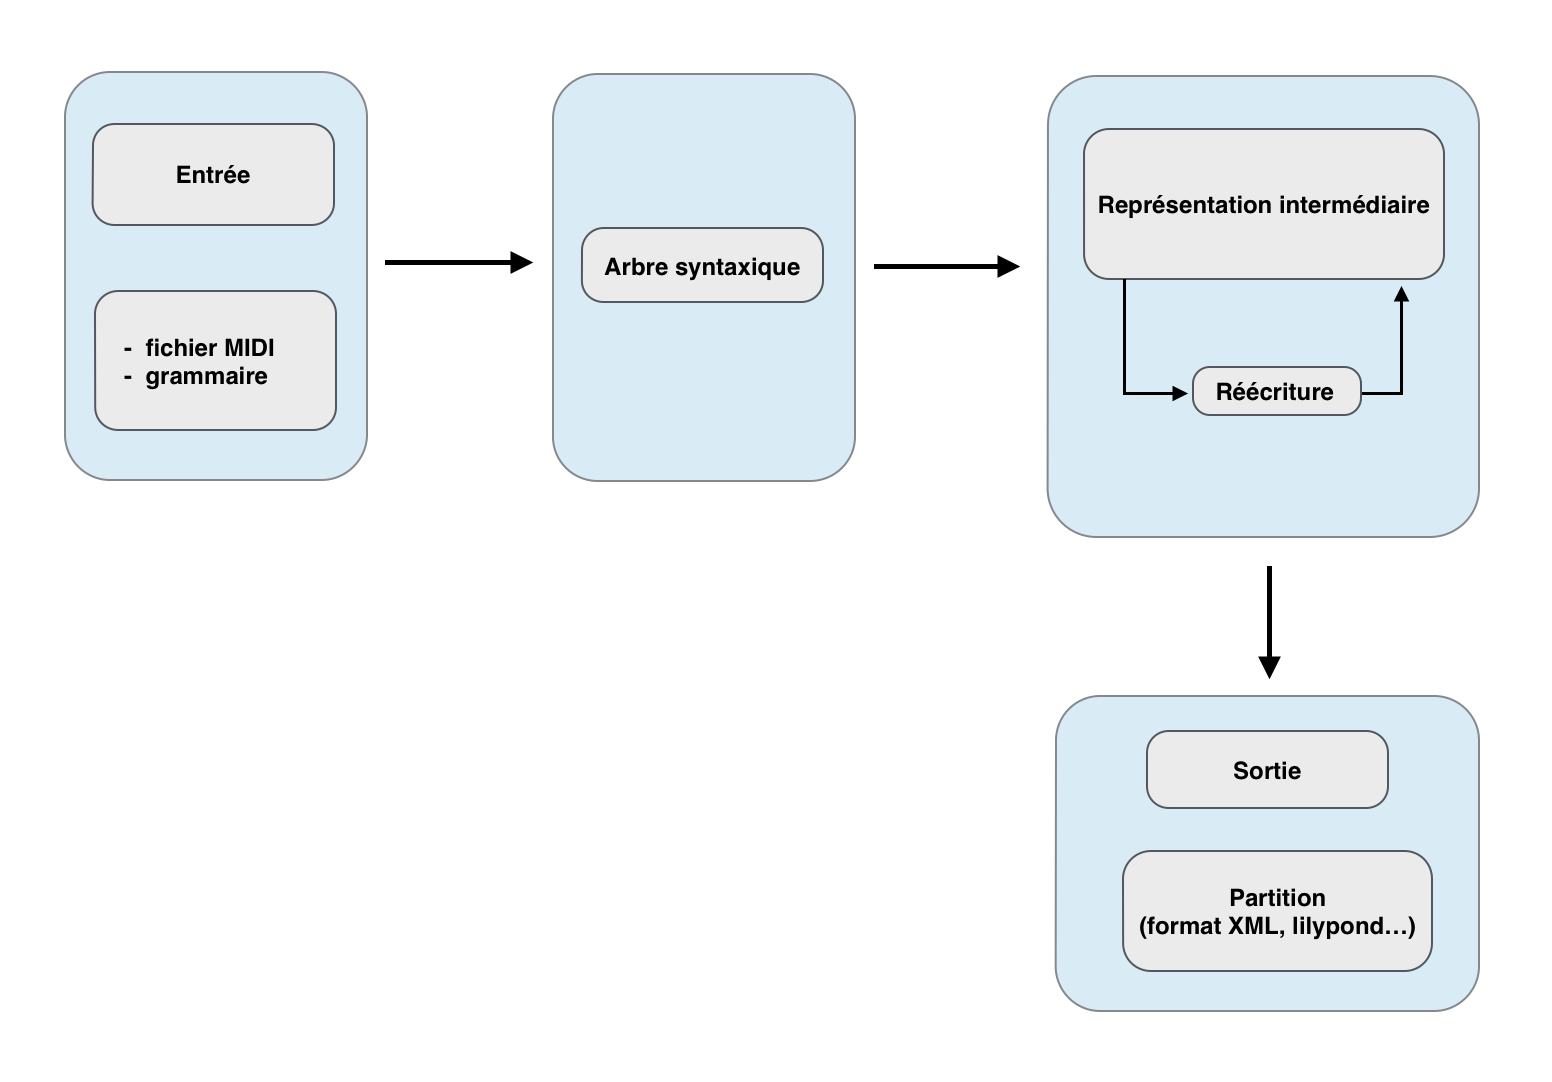
\includegraphics[height=70mm, width=110mm]{
z_images/3_methodes/1_Analyse_syntaxique/schema_qparse.png}
\caption{Présentation de Qparse}
\label{presentation_qparse}
\end{figure}

Comme le montre la figure \ref{presentation_qparse}, qparse\footnote{
\url{https://qparse.gitlabpages.inria.fr}} est un outil pour la transcription
musicale, qui, à partir d'une performance symbolique, séquentielle et non
quantifiée, produit une partition structurée. Il effectue conjointement des
tâches de quantification rhythmique et d'inférence de la structure de la
partition à l'aide de techniques d’analyse syntaxique (\textit{parsing}). Le
but du \textit{parsing} est en effet la structuration d'une représentation
séquentielle en entrée (un mot fini), suivant un modèle de langage
\cite{grune2007parsing}.

Dans le cas de qparse, le "mot" d'entrée est typiquement au format MIDI, et le
modèle de langage est une grammaire d'arbres pondérés représentant des
préférences en terme de notation musicale à produire \cite{droste2009handbook}.
basée sur des algorithmes d'analyse syntaxique pour les grammaires
arborescentes pondérées. En prenant en entrée une performance musicale
symbolique (séquence de notes avec dates et durées en temps réel, typiquement
un fichier MIDI), et une grammaire hors-contexte pondérée décrivant un langage
de rythmes préférés, il produit une partition musicale. Plusieurs formats de
sortie sont possibles, dont les formats XML (MEI, MusicXML,…), lilypond,…

Les principaux contributeurs sont :
\begin{itemize}
	\item Florent Jacquemard (Inria) : développeur principal.
	\item Francesco Foscarin (PhD, CNAM) : apprentissage ; Evaluation.
	\item Clement Poncelet (Salzburg U.) : integration de la librairie Midifile
        pour les input MIDI.
	\item Philippe Rigaux (CNAM) : production de partition au format MEI et de
        modèle intermédiaire de partition en sortie.
	\item Masahiko Sakai (Nagoya U.) : mesure de la distance input/output pour
        la quantification et CMake framework ; évaluation.
\end{itemize}

\subsection*{Les enjeux}
Plusieurs enjeux : <dam>idem à rédiger je suppose... un assez gros morceau
puisqu'il contiendra une partie de ta problématique appliquée</dam>
Le problème du MIDI avec Qparse\\
ON-OFF en entrée $\Rightarrow$ 1 seul symbole en sortie.\\
Minimiser la distance entre le midi et la représentation en arbre.\\
Un des problèmes de Qparse était qu’il était limité au monophonique.\\
Quelles sont les limites du monophonique ?\\
Impossibilité de traiter plusieurs voix et de reconnaître les accords.

\subsection*{La grammaire}
Il s’agit d’une grammaire hors-contexte pondérée…
<dam>incompréhensible ainsi, c'est dommage</dam>
// bar level\\
0 -> C0                1\\
0 -> E1                1\\
0 -> U4(1, 1, 1, 1)    1\\

// half bar level\\
9 -> C0                1\\
9 -> E1                1\\

// beat level\\
1 -> C0                1\\
1 -> E1                1\\
1 -> T2(2, 2)          1\\
1 -> T4(4, 4, 4, 4)    1\\

// croche level\\
2 -> C0                1\\
2 -> E1                1\\

// double level\\
4 -> C0                1\\
4 -> E1                1\\
4 -> E2                1\\
4 -> T2(6, 6)          1\\

// triple level\\
6 -> E1                1\\\\
Cette grammaire sépare les ligatures par temps au niveau de la mesure. Puis, au
niveau du temps, elle autorise les divisions par deux (croches) et par quatre
(doubles-croches). Tous les poids sont réglés sur 1. L’arbre de parsing en
résultant est considéré comme « convaincant » car il découpe correctement les
mesures et les temps.

\subsection*{Le parsing}
Les données MIDI sont quantifiées, les notes de dates proches sont alignées et
les relations entre les notes sont identifiées (accords, fla, etc…) ; un arbre
syntaxique global est créé ;

\subsection*{La représentation intermédiaire}
\begin{itemize}
    \item Les pitchs sont remplacés par les codes des instruments (voir tableau
    \ref{nom_instru_batt} ;
    \item réécriture 1 :\\
    séparation des voix $\Rightarrow$ un arbre par voix
    $\Rightarrow$ représentation intermédiaire (RI) ;
    \item réécriture 2 :\\
    simplification de l’écriture de chaque voix dans la RI.
    <dam>rédiger un peu mieux réécriture 1 et 2</dam>
\end{itemize}

\section{Les \textbf{formes rythmiques}}
\label{systemes_methodes}
Il existe en batterie des motifs rythmiques répétés (joués en boucle). Ces
motifs sont le résultat de la coordination de plusieurs instruments de la
batterie, je les nommerai \textbf{motifs} dans la suite du document. Très
souvent, un autre instrument est joué de manière indépendante sur le
\textbf{motif} mais en respectant la cohérence rythmique du \textbf{motif}. Je
nommerai \textbf{gamme} l’ensemble des combinaisons possibles pour cet autre
instrument. La \textbf{gamme} d’un \textbf{motif} est toujours relative à sa
signature rythmique. Enfin, j’ai nommé \textbf{forme rythmique} (\textbf{FR})
le couple \textbf{motif}-\textbf{gamme}.

\subsection*{Objectifs}
Le but est d'avoir des schemas types (les \textbf{formes rythmiques}) pour
calculer la séparation en voix. Cela constituerait une heuristique pour éviter
d'avoir à explorer une grande combinatoire.

Un ensemble de \textbf{formes rythmiques} comprenant leur signatures rythmiques
respectives et leurs règles spécifiques de réécriture sera nécessaire.

Une fois un système défini, la transcription à partir de l'entrée MIDI sera
facilitée par la reconnaissance de la FR qui contraindra le processus, il
premettra de :
\begin{itemize}
	\item définir une signature rythmique ;
	\item choisir une grammaire appropriée ;
	\item fournir les règles de réécriture (séparation des voix et
        simplification.
\end{itemize}

\subsection*{Définitions}

\begin{itemize}
    \item \textbf{motif} : rythmes coordonnés joués avec deux ou trois
        instruments coordonnés en boucle (répartis sur 1 ou 2 voix) ;
    \item \textbf{gamme} : Ensemble des combinaisons jouées par un autre
        instrument sur le \textbf{motif} (réparti sur 1 voix) ;
    \item \textbf{forme rythmique} : \textbf{motif} + \textbf{gamme}\\
\end{itemize}

Les \textbf{motifs} sont fixes, contrairement aux \textbf{gammes} regroupent
l’ensemble des possibilités qui peuvent être rencontrées en situation réelle
(sur une partition ou lors d’une performance de batterie).

Un \textbf{motif} détermine la signature rythmique d’une
\textbf{forme rythmique} , et donc de sa \textbf{gamme}. Il détermine aussi
avec quel instrument unique sera jouée la \textbf{gamme} et comment tous les
instruments de la \textbf{forme rythmique} se répartiront en voix.\\




Les \textbf{formes rythmiques} devront être distribuées dans 4 grandes
catégories\footnote{SR du tableau signifie « signature rythmique »}
\cite{system_drums} :
\begin{table}[h]
\centering
\begin{tabular}{|c|c|c|c|c|} \hline
\textbf{FR} & SR & Subdivisions & Possibles & nb
voix \\ \hline
binaires & simple & doubles-croches & triolets, sextolets & 2 \\
jazz & simple & triolets & croches et doubles & 2 \\
ternaires & complexe & croches & duolets, quartelets & 2 \\
afros-cubains & simple & croches & - & 3 \\ \hline
\end{tabular}
\caption{Sytèmes}
\end{table}\\
Nous exposerons 3 \textbf{formes rythmiques} afin d’illustrer les propos de
cette section :
\begin{itemize}
	\item 4/4 binaire 
	\item 4/4 jazz
	\item 4/4 afro-cubain
\end{itemize}

Le \textit{\textbf{motif}} et la

\subsubsection{Détection de la signature rythmique}
La partie \textbf{motif} des \textbf{FR} sera utilisée pour la
\textbf{définition des signature rythmiques}. 
La détection de la signature rythmique est importante, 
non seulement pour connaître le nombre de temps par mesure ainsi que le nombre
de subdivisions pour chacun de ces temps, mais aussi pour savoir comment écrire
l’unité de temps et ses subdivisions.

\begin{figure}[h]
	\centering
	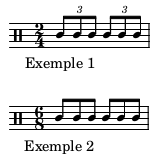
\includegraphics[height=40mm, width=40mm]{
    z_images/3_methodes/2_systemes/0_simple_VS_complexe.png}
	\caption{signature rythmique}
	\label{subdivisions}
\end{figure} %\newpage

La figure \ref{subdivisions} montre deux signatures rythmiques différentes. 
L’une (exemple 1) est \textit{simple} (2 temps binaires sur lesquels sont joués
des triolets), l’autre (exemple 2) est \textit{complexe} (2 temps ternaires). 
Le jazz est traditionnellement écrit en binaire avec ou sans triolet (même si
cette musique est dite ternaire alors que le rock ternaire sera plutôt écrit
comme dans l’exemple 2).

\subsubsection{Choix d’une grammaire}
Il faut prendre en compte l’existence potentielle de plusieurs grammaires
qui regroupent les contenus MIDI par signature rythmique. Le choix d’une
grammaire pondérée doit être fait avant le parsing puisque qparse prend en
entrée un fichier MIDI et un fichier wta (grammaire). C’est pour cette raison
que la signature rythmique doit être définie avant le choix de la grammaire.
Il faudrait les trouver automatiquement sans autres indications que les
contenus MIDI. Par conséquent, les \textbf{motifs} des
\textbf{formes rythmiques} devront être recherchés sur l’input (fichiers MIDI)
avant le lancement du parsing, afin de déterminer la signature rythmique en
amont. Cette tâche devra probablement être effectuée par utilisation
d'apprentissage automatique.


\subsubsection{Séparation des voix}

L’objectif de la procédure : ?

Le principe de la procédure : ?

Quelles sont les difficultés et les choix de séparation de voix et comment un
algorithme pourrait faire ces choix ?

\label{sys_sep_voix}
\begin{figure}[h]
	\centering
	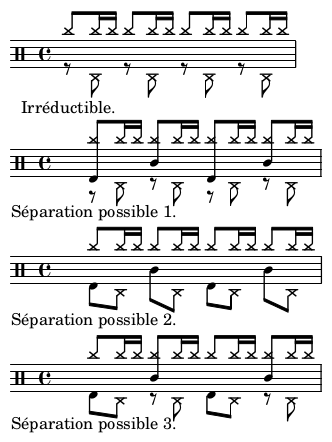
\includegraphics[height=60mm, width=40mm]{
    z_images/3_methodes/2_systemes/1_separation_4-4_binaire.png}
	\caption{\textbf{motif} 4-4 binaire}
	\label{binaire}
\end{figure}


Ici, la \textbf{forme rythmique} est construite sur un modèle rock avec une
signature rythmique en 4/4.

La première ligne de la figure \ref{binaire} est
appelée « Irréductible » car il n’y a pas d’autre choix de séparation des voix
pour la ride et le charley au pied.

La troisième séparation proposée est privilégiée car elle répartit selon deux 
voix, une voix pour les mains (ride et caisse claire) et une voix pour les
pieds (charley et grosse caisse). Ce choix paraît plus équilibré car deux
instruments sont utilisés par voix (contrairement séparations possibles 1 et 2
de la figure \ref{binaire}) et plus logique pour le lecteur puisque les mains
sont en haut et les pieds en bas.

\begin{figure}[h]
\centering
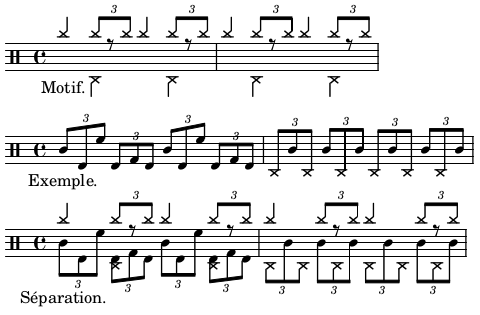
\includegraphics[height=45mm, width=60mm]{
z_images/3_methodes/2_systemes/2_separation_4-4_jazz.png}
\caption{\textbf{Motif} 4-4 jazz}
\label{jazz}
\end{figure}
\newpage
Dans la plupart des méthodes, le charley n’est pas écrit car il est considéré
comme évident en jazz traditionnel. Ici, le parti pris est de tout écrire.

Dans la figure \ref{jazz}, les mesures 1 et 2 de la ligne « Exemple » combinées
avec le \textbf{motif} de la première ligne, sont des cas typiques de la
batterie jazz. Tout mettre sur la voix haute serait surchargé. De plus, la
grosse caisse entre très souvent dans le flot des combinaisons de toms et de
caisse claire et son écriture séparée serait inutilement compliquée et peu
intuitive pour le lecteur. Le choix de séparation sera donc de laisser les
cymbales jouées à la main en haut, et les toms, la caisse claire, la grosse
caisse et la pédale de charley en bas.

\begin{figure}[h]
	\centering
	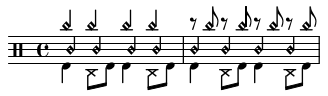
\includegraphics[height=20mm, width=70mm]{
    z_images/3_methodes/2_systemes/3_separation_afro-latins.png}
	\caption{\textbf{Forme rythmique} 4-4 afro-latin}
	\label{afro_latin}
\end{figure}

La figure \ref{afro_latin} montre un exemple minimaliste de
\textbf{forme rythmique} afro-latin \cite{system_drums}.

Cette \textbf{forme rythmique} doit être écrite sur trois voix car la voix
centrale est souvent plus complexe que sur la figure et la mélanger avec le
haut ou le bas serait surchargé et peu lisible.

\subsubsection{Simplification de l’écriture}

Les règles de \textbf{simplification} (les combinaisons de réécritures) seront
extraites des voix séparées des \textbf{formes rythmiques}.
Les explications qui suivent seront appuyées par une réécriture guidée dans la
section \ref{reecriture_guidee}.

Les \textbf{gammes} qui accompagnent les \textbf{motifs} étayent toutes les
combinaisons d’un \textbf{FR} et elles permettent, combinées avec le
\textbf{motif}, de définir ses propres règles de simplification.\\

Voici les différentes étapes à suivre :
\begin{itemize}
	\item pour chaque \textbf{gamme} d’une \textbf{forme rythmique}, faire un
        arbre de rythme représentant la \textbf{gamme} combinée avec le
        \textbf{motif} de la \textbf{FR} ;
	\item pour chaque arbre de rythmes obtenus, séparer les voix et faire un
        arbre de rythme par voix ;
	\item pour chaque voix (arbres de rythmes) obtenus, extraire tous les nœuds
        qui nécessitent une simplification et écrire la règle.\\
\end{itemize}

Certaines précisions concernant l’extraction de ces règles sont nécessaires. 
Il s’agit de précisions à propos de la durée, des silences et de la présence ou
non d’ouvertures de charley dans les instruments joués. 
Nous avons discuté de ces problèmes plus haut dans ce chapitre.\\

Voici quelques règles inhérentes à la simplication de l’écriture pour la
batterie :

Même si on favorise l’usage des silences pour l’écart entre les notes
n’appartenant pas au même temps, on les remplace systèmatiquement par un point
pour 2 notes au sein d’un même temps.

\begin{figure}[h]
	\centering
	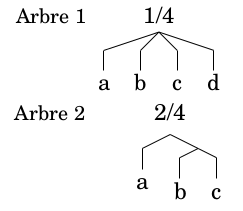
\includegraphics[height=45mm, width=50mm]{
    z_images/3_methodes/2_systemes/simplification_0.png}
	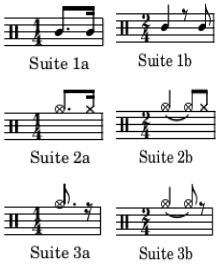
\includegraphics[height=50mm, width=40mm]{
    z_images/3_methodes/2_systemes/simplification_2.png}
	\caption{Simplifications — arbres et notations possibles}
	\label{simpl}
\end{figure}

Dans la figure \ref{simpl}, les « suites » sont des notations possibles
relatives aux arbres 1 ou 2.\\

\textit{Rappel :\\cf = charley fermé joué à la main ;\\co = charley ouvert joué
à la main ;\\ pf = charley fermé joué au pied.}\newpage

Soit l’arbre 1 de la figure \ref{simpl} dans lequel :
\begin{itemize}
    \item a et d sont des instruments de la batterie (x) ;
    \item b et c sont des continuations (t).
\end{itemize}
Pour chacune des conditions suivantes, une suite de la
figure \ref{simpl} est attribuée :
\begin{itemize}
	\item Si a n’est pas un co :\\
	$\Rightarrow$ Suite 1a.
	\item Si a est un co :
	\begin{itemize}
		\item Si d est un cf :\\
		$\Rightarrow$ Suite 2a.
		\item Si d est un pf :\\
		$\Rightarrow$ Suite 3a : d deviens un silence (r).\\
	\end{itemize}
\end{itemize}
Soit l’arbre 2 de la figure \ref{simpl} dans lequel :\\
a et c sont des instruments de la batterie (x) ;\\
b est une continuation (t) ;
Pour chacune des conditions suivantes, une suite de la figure \ref{simpl} est
attribuée :
\begin{itemize}
	\item Si a n’est pas un co :\\
	$\Rightarrow$ Suite 1b, b devient un silence.
	\item Si a est un co :
	\begin{itemize}
		\item Si c est un cf :\\
		$\Rightarrow$ Suite 2b, b devient une liaison et c devient un cf.
		\item Si c est un pf :\\
		$\Rightarrow$ Suite 3b : b deviens une liaison et c devient un silence.
	\end{itemize}
\end{itemize}

\section*{Conclusion}
Dans ce chapitre, nous avons formalisé une notation de la batterie inspirée des
méthodes de batterie Dante Agostini, modélisé cette notation pour
la transcription de données MIDI en partition.
Nous avons ensuite parlé de l’outil utilisé pour les transcriptions manuelles
en mettant en avant que cet outil devrait être utilisé pour la transcription de
la batterie et en précisant que tous les codes lilypond pour la création des
figures et partition de ce mémoire sont en accès libre sur github. Nous avons
ensuite décrit qparse qui l’outil que le travail de ce mémoire cherche à
améliorer.

Enfin, nous avons exposé une approche de type dictionnaire (les « formes
rythmiques ») pour détecter une signature rythmique, choisir une grammaire
pondérée appropriée et énoncer des règles de séparation des voix et de
simplification de l’écriture.
